\begin{figure*}[t]
\centering
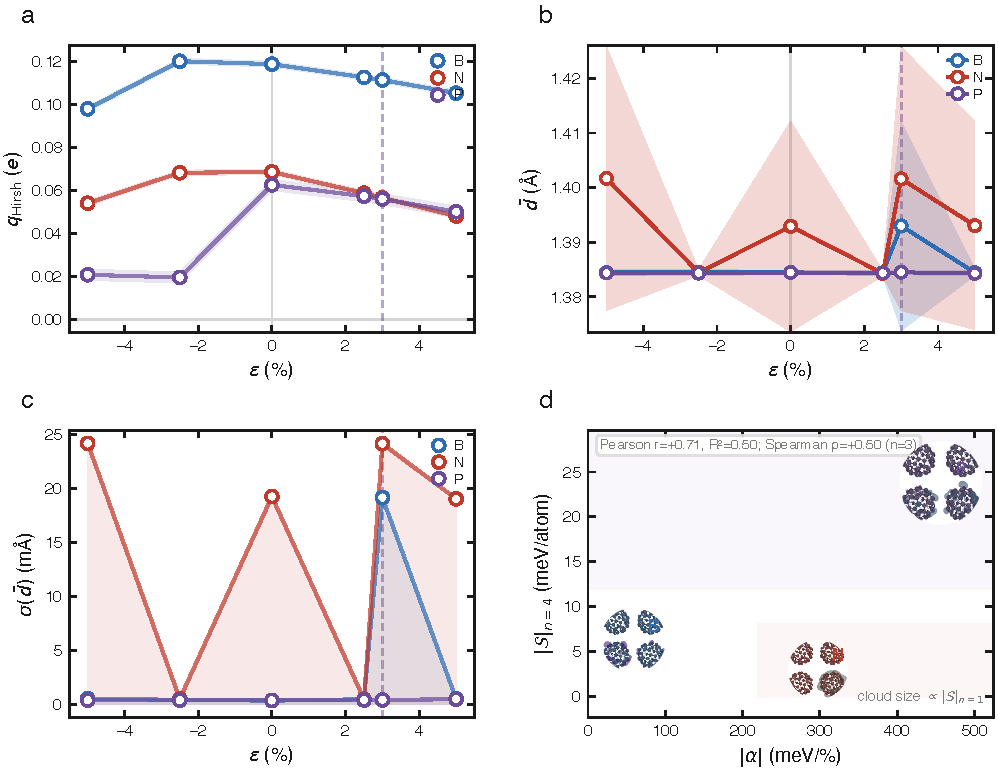
\includegraphics[width=\textwidth]{figures/out/figure_prb_3_decoupling.pdf}
\caption{\label{fig:decoupling}Microscopic strain paths and $\alpha$--$|\mathcal{S}|$ rank comparison ($n{=}3$ dopants).
(a)~Hirshfeld $q(\epsilon)$ for B/N/P (six-point paths; dotted guide at $+3$\%).
(b)~Nearest-neighbor $\bar{d}(\epsilon)$ with $\pm\sigma$ bands.
(c)~Local disorder path $\sigma(\bar{d})(\epsilon)$.
(d)~Reference-map $|\alpha|$ vs.\ periodic $|\mathcal{S}|_{n=4}$ (marker area $\propto|\mathcal{S}|_{n=1}$; horizontal bars: linear-fit standard errors on the six-point strain grid).
N inverts a naive $|\alpha|\rightarrow|\mathcal{S}|$ expectation; with only three dopants this panel reports qualitative ranking, not Pearson, $R^2$, or Spearman statistics.}
\end{figure*}
